% David Sánchez Jiménez
% davidsanchezjimenez@correo.ugr.es

\documentclass[10pt,a4paper,spanish]{report}

\usepackage[spanish]{babel}
\usepackage[utf8]{inputenc}
\usepackage{amsmath, amsthm}
\usepackage{amsfonts, amssymb, latexsym}
\usepackage{enumerate}
\usepackage[official]{eurosym}
\usepackage{graphicx}
\usepackage[usenames, dvipsnames]{color}
\usepackage{colortbl}
\usepackage{multirow}
\usepackage{fancyhdr}
\usepackage{fancybox}
\usepackage{pseudocode}
\usepackage[all]{xy}
\usepackage{minted}
\usepackage{tikz}
\usepackage{pgfplots}

\pgfplotsset{compat=1.5}

% a4large.sty -- fill an A4 (210mm x 297mm) page
% Note: 1 inch = 25.4 mm = 72.27 pt
%       1 pt = 3.5 mm (approx)

% vertical page layout -- one inch margin top and bottom
\topmargin      0 mm    % top margin less 1 inch
\headheight     0 mm    % height of box containing the head
\headsep       10 mm    % space between the head and the body of the page
\textheight   250 mm
\footskip      14 mm    % distance from bottom of body to bottom of foot

% horizontal page layout -- one inch margin each side
\oddsidemargin    0   mm    % inner margin less one inch on odd pages
\evensidemargin   0   mm    % inner margin less one inch on even pages
\textwidth      159.2 mm    % normal width of text on page

\usepackage[math]{iwona}
\usepackage[T1]{fontenc}
\usepackage{inconsolata}

\usepackage[pdftex, bookmarks=true,
bookmarksnumbered=false, % true means bookmarks in
% left window are numbered
bookmarksopen=false,     % true means only level 1
% are displayed.
colorlinks=true,
linkcolor=webblue]{hyperref}

\definecolor{webgreen}{rgb}{0, 0.5, 0} % less intense green
\definecolor{webblue}{rgb}{0, 0, 0.5}  % less intense blue
\definecolor{webred}{rgb}{0.5, 0, 0}   % less intense red
\definecolor{dblackcolor}{rgb}{0.0,0.0,0.0}
\definecolor{dbluecolor}{rgb}{.01,.02,0.7}
\definecolor{dredcolor}{rgb}{0.8,0,0}
\definecolor{dgraycolor}{rgb}{0.30,0.3,0.30}

\newcommand{\HRule}{\rule{\linewidth}{0.5mm}}

\pagestyle{fancy}

\renewcommand{\chaptermark}[1]{%
\markboth{#1}{}}
\renewcommand{\sectionmark}[1]{%
\markright{\thesection\ #1}}
\fancyhf{}
\fancyhead[LE,RO]{\bfseries\thepage}
\fancyhead[LO]{\bfseries\leftmark}
\renewcommand{\headrulewidth}{0.5pt}
\renewcommand{\footrulewidth}{0pt}
\addtolength{\headheight}{0.5pt}
\fancypagestyle{plain}{
\fancyhead{}
\renewcommand{\headrulewidth}{0pt}
}

\title{\textbf{Práctica 4 FIS}}
\author{Laura Gómez Garrido\\
		Javier Sáez Maldonado\\
		Daniel Pozo Escalona\\
		Luis Ortega Andrés}

\usepackage{sectsty}
\chapterfont{\fontfamily{pag}\selectfont}
\sectionfont{\fontfamily{pag}\selectfont}
\subsectionfont{\fontfamily{pag}\selectfont}
\subsubsectionfont{\fontfamily{pag}\selectfont}

\renewcommand{\labelenumi}{\arabic{enumi}. }
\renewcommand{\labelenumii}{\labelenumi\alph{enumii}) }
\renewcommand{\labelenumiii}{\labelenumii\roman{enumiii}: }

\begin{document}


\maketitle

\section*{Parte Javier}
\subsection*{terminarConsulta(idMedico,idPaciente)}
\begin{center}
	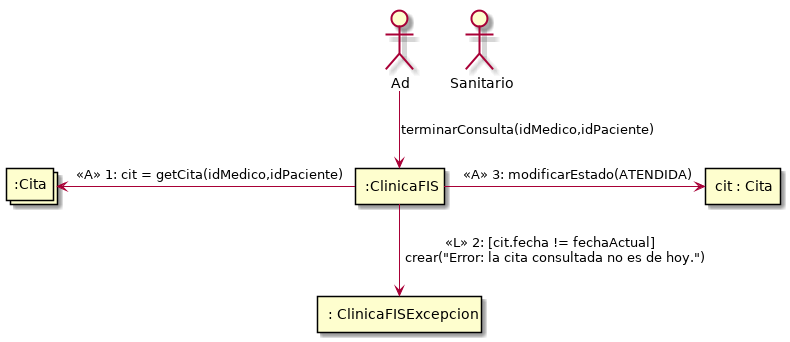
\includegraphics[scale=0.6]{terminarConsulta.png}
\end{center}

\subsection*{infoDiagnostico = diagnosticar(idHC, codDiagnostico, textoExplicativo, 
idMedico)}
\begin{center}
	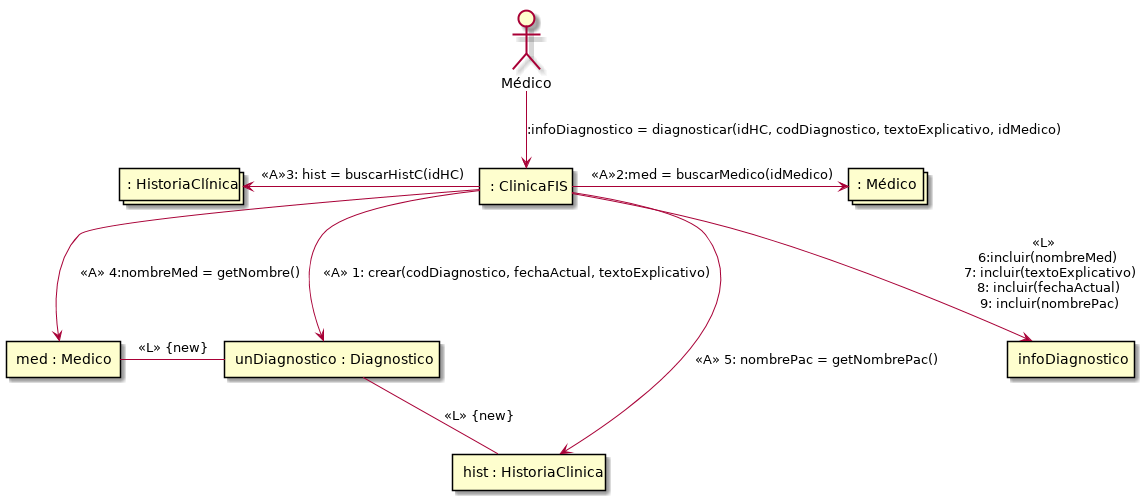
\includegraphics[scale=0.4]{diagnosticar.png}
\end{center}

\subsection*{infoPaciente = consultarPaciente(idPaciente)}
\begin{center}
	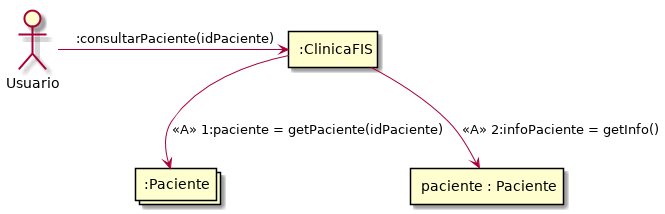
\includegraphics[scale=0.6]{infoPaciente.png}
\end{center}



\section*{Parte Laura}

\subsection*{}
\begin{center}
	
\end{center}
\subsection*{}
\begin{center}
	
\end{center}
\subsection*{}
\begin{center}
	
\end{center}
\section*{Parte Daniel}
\subsection*{}
\begin{center}
	
\end{center}
\subsection*{}
\begin{center}
	
\end{center}
\subsection*{}
\begin{center}
	
\end{center}
\section*{Parte Luis}
\subsection*{}
\begin{center}
	
\end{center}
\subsection*{}
\begin{center}
	
\end{center}
\subsection*{}
\begin{center}
	
\end{center}

\end{document}
